\chapter{Automation Fundamentals for IT Consultants}


\section{Introduction}

As a small IT consulting firm, your time is your most valuable asset. In this chapter, we'll dive into a practical automation example that can save you hours each week and revolutionize how you handle client communications.


\section{Quick Win: AI-Powered Email Classification with n8n and OpenAI}

Let's start with a common pain point: the overflowing inbox. We'll create an automation that reviews and classifies emails based on their content, helping you prioritize and respond more efficiently.

We will solve that in this chapter.

\subsection{Why This Matters}

\begin{figure}[h]
    \centering
    [@TODO: ILLUSTRATATE: Cluttered inbox vs. Organized, classified inbox]
    \caption{Cluttered inbox vs. Organized, classified inbox}
\end{figure}

Imagine starting your day with a perfectly organized inbox, where emails are automatically sorted into categories like:

\begin{itemize}
    \item Urgent client issues
    \item Project updates
    \item New business inquiries
    \item Invoicing and payments
    \item Administrative tasks
\end{itemize}

This automation will make that a reality, allowing you to:
\begin{itemize}
    \item Respond to critical issues faster
    \item Prioritize your workday more effectively
    \item Ensure no important client communication slips through the cracks
\end{itemize}

Here's going to be our flow:

\begin{figure}
    \centering
    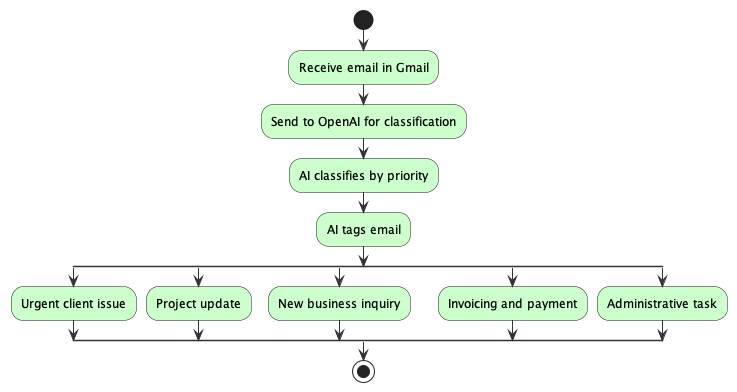
\includegraphics[width=0.8\textwidth]{./figures/01-n8n-flow}
        \caption{Email Classification and Tagging Automation Flow}
    \label{fig:01_email_automation}
\end{figure}


\section{Setting Up Your Secure Automation Environment}

Before we dive into the automation itself, let's set up n8n locally. Unlike cloud-based tools like Zapier, n8n can be self-hosted, ensuring your sensitive client data never leaves your control.

\subsection{Installing n8n using Docker}

We'll use Docker for a consistent setup across all platforms.

\begin{enumerate}
    \item Install Docker:
    \begin{itemize}
        \item For Windows: Docker Desktop for Windows
        \item For macOS: Docker Desktop for Mac
        \item For Linux: Docker Engine
    \end{itemize}
    \item With the installation complete, open a terminal or command prompt and run:
    \begin{lstlisting}[language=bash, label={lst:n8n-docker-run}]
docker run -it --rm \
  --name n8n \
  -p 5678:5678 \
  -v ~/.n8n:/home/node/.n8n \
  n8nio/n8n
    \end{lstlisting}
    \item Open your browser and navigate to \url{http://localhost:5678}, you should see the setup screen: \newline
    \begin{minipage}[t]{\linewidth}
        \raggedright
        \adjustbox{valign=t}{%
            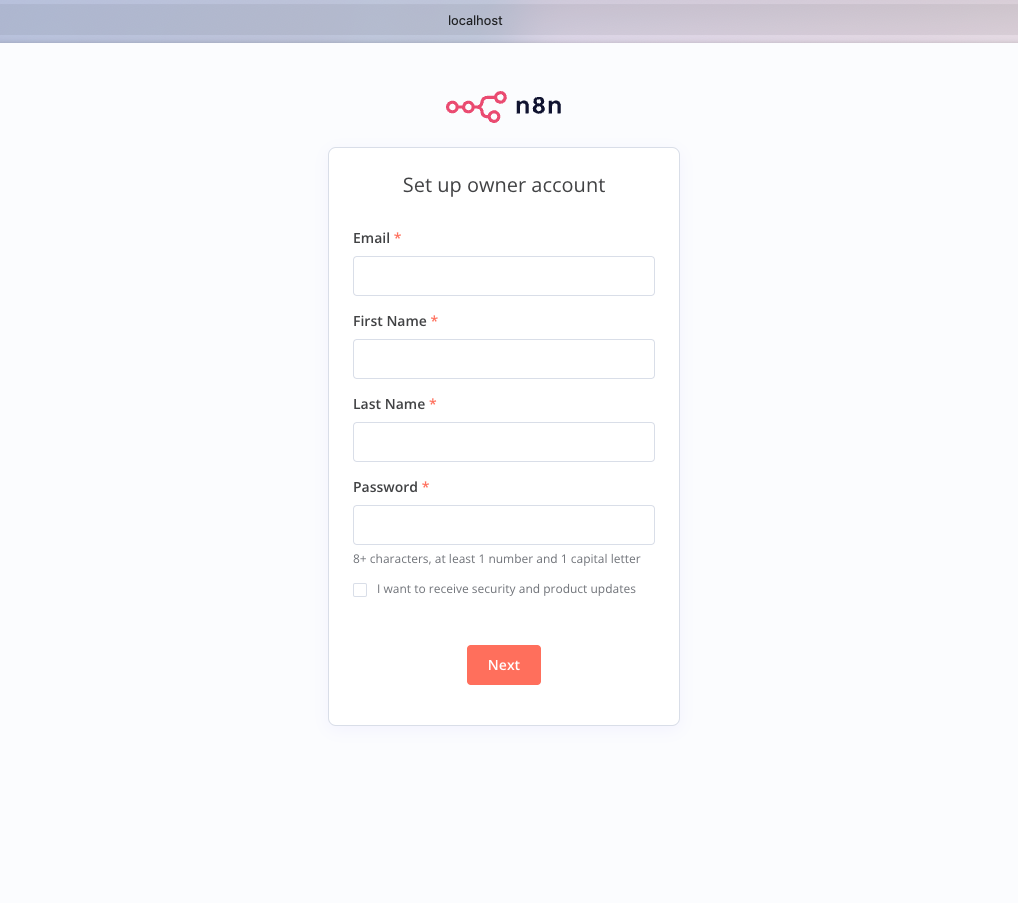
\includegraphics[width=1\linewidth]{./figures/01-n8n-startscreen}%
        }
        \medskip
    \end{minipage}
    \item  Fill in your details and hit "Next"
\end{enumerate}


\importantbox{If you run into issues in your setup and want to restart from the beginning, from your terminal, delete the docker n8n directory in ~/.n8n. Then re-run the docker command}


\section{Creating Your Email Classification Workflow}

Now that n8n is running, let's build our automation:

\begin{enumerate}
    \item In the n8n dashboard, click "Start from scratch"
    \item Rename "My Workflow" in the top left corner to "Email Classifier"
    \begin{minipage}[t]{\linewidth}
        \raggedright
        \adjustbox{valign=t}{%
            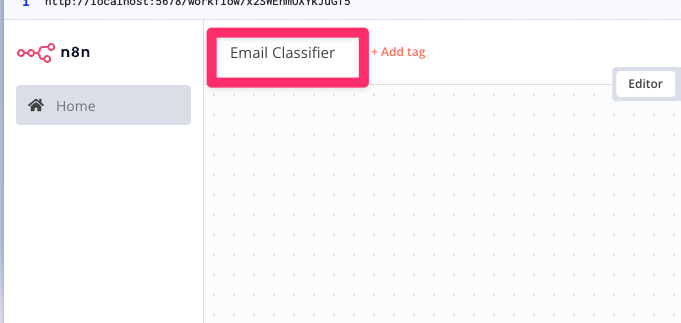
\includegraphics[width=1\linewidth]{./figures/01-n8n-rename-workflow}%
        }
        \medskip
    \end{minipage}

\end{enumerate}

\subsection{Step 1: Connect to Gmail}

\begin{enumerate}
    \item Hit the "Add first step..." and Search for "Gmail" and select "On Message Received"
    \item Select the "Credential to connect with" then choose "- Create New Credential -"
    \item Follow the OAuth process to connect your Gmail account
  \end{enumerate}

\begin{figure}[h]
    \centering
    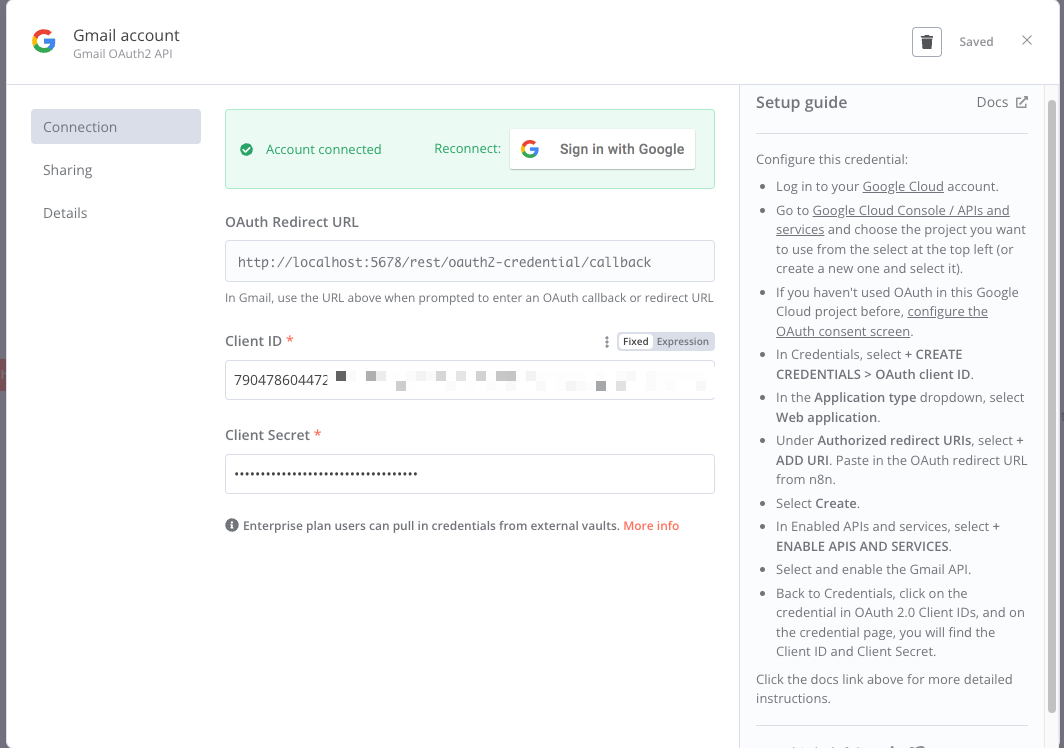
\includegraphics[scale=0.35]{./figures/01-n8n-gmail-oauth-config}
    \caption{The Complete OAuth config screen}
    \label{fig:01-gmail-config}
\end{figure}

\subsection{Step 2: Integrate OpenAI for Content Analysis}

Before we proceed, let's securely set up our OpenAI API access:

\begin{enumerate}
    \item Go to OpenAI's website and sign up or log in
    \item Navigate to the API section and create a new API key
    \item In n8n, go to Settings > Credentials and add a new credential of type "OpenAI API"
    \item Paste your API key and save
\end{enumerate}

Now, let's add the OpenAI node to our workflow:

\begin{enumerate}
    \item Add a new "OpenAI" node
    \item Connect it to the Gmail trigger node
    \item Configure it as follows:
    \begin{itemize}
        \item Resource: Completion
        \item Model: gpt-4o
        \item Prompt: "Classify the following email into one of these categories: Urgent client issue, Project update, New business inquiry, Invoicing and payment, Administrative task. Email content: \{\{\$json["body"]\}\}"
        \item
    \end{itemize}
\end{enumerate}

\begin{figure}[h]
    \centering
    [INSERT IMAGE: OpenAI node configuration]
    \caption{OpenAI node configuration}
\end{figure}

\subsection{Step 3: Update Email Labels}

\begin{enumerate}
    \item Add another "Gmail" node
    \item Connect it to the OpenAI node
    \item Configure it to add a label based on the classification from OpenAI
\end{enumerate}

\begin{figure}[h]
    \centering
    [@TODO: ILLUSTRATE: Final workflow diagram]
    \caption{Final workflow diagram}
\end{figure}


\section{Putting It All Together}

Activate your workflow, and watch as your emails are automatically classified and labeled!

\begin{figure}[h]
    \centering
    [@TODO: ILLUSTRATE: Before and after screenshots of a Gmail inbox]
    \caption{Before and after screenshots of a Gmail inbox}
\end{figure}


\section{Real-World Impact: A Case Study}

Meet Sarah, an use-case IT consultant running a 5-person firm. Before implementing this automation, Sarah spent 2 hours each day sorting through emails. After setting up the AI-powered classification:

\begin{itemize}
    \item Sarah's email processing time dropped to 30 minutes a day
    \item Her team's response time to urgent client issues improved by 60\%
    \item They never missed a new business inquiry, increasing potential leads by 25\%
\end{itemize}

By reclaiming 7.5 hours each week, Sarah was able to take on two additional clients without hiring new staff.


\section{Next Steps and Community Support}

Ready to implement this automation or explore more advanced use cases? Join our vibrant community of IT consultants and automation enthusiasts on Discord:

JOIN NOW: \href{https://discord.gg/P6txNctp}{Business Automators Discord Server}

In our community, you can:
\begin{itemize}
    \item Get help troubleshooting your automations
    \item Share your own automation success stories
    \item Network with other forward-thinking IT consultants
    \item Get direct access to me, Dele Tosh, for personalized advice
\end{itemize}

Remember, automation is a journey, not a destination. Start with this email classification workflow, then explore how you can automate other aspects of your consulting practice. In the next chapter, we'll dive deeper into the no-code tools every IT consultant should master.